\documentclass[a4paper]{article}

\usepackage[a4paper,top=0.4in,left=0.4in,right=0.4in,bottom=0.4in]{geometry}
\usepackage{graphicx}
\usepackage{rotating}
\usepackage{hyperref}
\usepackage{multirow}
\usepackage{setspace}
\usepackage{float}
\usepackage{caption}
\usepackage{subfigure}


\usepackage{tabularx,ragged2e,booktabs,caption}
\newcolumntype{C}[1]{>{\Centering}m{#1}}
\renewcommand\tabularxcolumn[1]{C{#1}}

\usepackage{titling}

\graphicspath{ {./images/} }


\begin{document}

\linespread{1.5}


\input{cover}
\begin{flushleft}
{\setstretch{0.75}
\section{Aim}
Our team, \emph{Deadline Fighters}, set out with the aim to develop a multi-host file synchronizer which can:
\begin{itemize}
\item{allow upload and download of files from a central server (hub) through client applications with necessary authorization.}
\item{automatically synchronize changes made by client applications unto the corresponding copy of the file in the server.}
\item{handle all possible conflict/non-conflict scenarios of file synchronization (ie. combinations of Create, Edit, Rename, Delete) involving multiple client applications.}
\item{enable file sychronization through both desktop (all platform) and mobile (Android) clients.}
\end{itemize}

The desktop application is developed using Electron framework to enable cross-platform compatibility. Based on feedback received during the preliminary presentation, we have developed a Python server with which our client applications interact. Python server, in turn, uses AWS S3 for storage and other purposes.

Of the above mentioned aims, we have been able to accomplish most of it with the following changes/exceptions:

\begin{itemize}
	\item{There is no authorization mechanism present on client applications, except for knowing which IP address to access. Python server, on the other hand, makes requests to AWS S3 after authentication.}
	\item{Automatic synchronization has been achieved using FileObserver libraries. It works well for regular use cases and bugs have been logged for other cases.}
	\item{Basic dev-tested conflict resolution mechanism implemented using ETag for files as created by AWS S3.}
\end{itemize}

Also, some effort have been put into the aesthetics and usability of the application UI using CSS.\newline

\begin{figure}[h!]
\centering
\includegraphics[scale=0.5]{User_use_case}

\caption{Functionalities provided by Deadline fighter application to Users}
\end{figure}


\newline 
The following are links to documentations that we have referenced during this project. All links were accessed during the period January 18, 2019 to March 28, 2019.

\begin{thebibliography}{9}

\bibitem{Amazon S3 SDK - Javascript}
Amazon S3 SDK for Javascript,
\textit{\url{https://docs.aws.amazon.com/AWSJavaScriptSDK/latest/AWS/S3.html}}

\bibitem{Amazon S3 SDK - Python}
Boto3 for S3 on Python,
\textit{\url{https://boto3.amazonaws.com/v1/documentation/api/latest/reference/services/s3.html}}

\bibitem{Upload files on S3}
Upload files on S3,
\textit{\url{https://blog.csdn.net/qq1147093833/article/details/80267542}}

\bibitem{Node.js and S3}
MyDatahack(2018),'Uploading and Downloading Files in S3 with Node.js'
\textit{\url{https://www.mydatahack.com/uploading-and-downloading-files-in-s3-with-node-js/}}

\bibitem{Server side Database}
SQLite Python, 'Tutorial for using Sqlite on Python',
\textit{\url{http://www.sqlitetutorial.net/sqlite-python/}}

\bibtiem{Tutorial}
Tutorial on API calls to AWS S3,
\textit{\url{https://grokonez.com/android/uploaddownload-files-images-amazon-s3-android#5_Connect_to_Amazon_S3}}

\bibitem{Android}
Upload to server using URL for Android,
\textit{\url{https://androidexample.com/Upload_File_To_Server_-_Android_Example/index.php?view=article_discription&aid=83}}

\bibitem{Listview}
Change listview height dynamically,
\textit{\url{https://stackoverflow.com/a/26501296}}

\end{thebibliography}
\section{System Design}
\subsection{Introduction}
The team \emph{Deadline Fighters} was given the overall requirement to build a ‘hub and spoke’ file synchroniser which has a single central server (the ‘hub’) to which multiple other clients (the ‘spokes’) can synchronise. The following are the operations that it entails and the priority of implementation we set for our team.

\bgroup
\def\arraystretch{1.3}
\begin{table}[H]
\centering
\begin{tabular}{|c|m{8cm}|c|c|}
\hline
Client name & User role & Priority & Description\\
\hline
{Desktop and Mobile} & View files on the server & 2 &{Priority description:} \\
\cline{2-3}
& Upload a file from local which is outside the local sync folder (only for Android)& 1&{}  \\
\cline{2-3}
& Upload a single file from local sync folder & 2&{\textbf{1-Highest priority}}\\
\cline{2-3}
& Upload multiple files from local sync folder & 2&{}\\
\cline{2-3}
&Download a single file from server & 1 &{(Important /necessary functions)}\\
\cline{2-3}
&Download multiple files from server & 2&{}\\
\cline{2-3}
&Reflect delete of a single file (Local to server) & 2&{}\\
\cline{2-3}
&Reflect delete of a single file (Server to local) & 2&{\textbf{4-Lowest priority}}\\
\cline{2-3}
&Reflect delete of multiple files (Local to server) & 3 &{}\\
\cline{2-3}
&Reflect delete of multiple files (Server to local) & 3&{(Will implement if time permits)}\\
\cline{2-3}
&Reflect rename (Local to server) & 2&{}\\
\cline{2-3}
&Reflect rename (Server to local) & 3&{}\\
\cline{2-3}
&Download edited changes on a single file from server & 3&{}\\
\cline{2-3}
&Download changes on two or more files from server & 4&{}\\
\cline{2-3}
&Synchronize all server and local files & 2&{}\\
\hline
\bottomrule
\end{tabular}
\caption{Functionalities to be enabled on client applications}
\end{table}
\egroup


\subsection{Architecture}

\begin{figure}[h!]
\centering
\includegraphics[scale=0.5]{Architecture}
\caption{Flow of operation across client, server and AWS S3}
\end{figure}


\subsection{Central server’s conflict role}
For central server: it will solve the conflict between multiple users operate at same time. The operate and resolution is shown as follow table.\newline
(Add conflict table here.)\newline
By using the conflict role as above in the file synchronisation tool development allows the system to reduce the number of error reports and make the system organized. It won't cause the system to lose files and report error when the user using two different synchronization functions at the same time to the server (eg. A client edit a file on the desktop application and the client delete the file on the mobile at the same time). It can avoid unnecessary data losses. Because the most important thing about a synchronous system is that you can't lose files. Through the table listed above, our team group can have a common standard for dealing with conflicts in the development process, making the development process more organized.\newline
According to the above detailed requirements design and contradictory solutions, it can help our team have a better assignment for the tasks to the team members and promote the teamwork. Team members can arrange their own time according to their own tasks to complete system functions implementation.\newline

\section{Implementation}

The initial team of 6 was divided into sub-teams of 2, each handling desktop client, mobile client and the server component. At this point, server component was AWS S3 and the client applications made direct calls. After team restructuring, development of local server began while the client applications continued to build the system to talk to AWS S3. Desktop, mobile and server code were pushed into corresponding feature branch and then merged into the master branch at regular intervals. This allowed for better testing and narrowing down of issues.\newline

Once the basic decisions about the server were made and functionalities implemented, client applications were migrated to interact through the local server. This delayed progress which we could have used into feature building if we had made better decisions on the server.\newline

Development process was agile with weekly scrum meetings on Thurdays. Emphasis was laid on writing maintainable features and code. Efforts were directed into code reviews, logging for client and server and documenting commonly faced issues. Bugs were tracked under \emph{issues} on our Git repository.\newline

The following are the versions of softwares, packages and IDEs used:\newline

\textbf{Desktop Application Development}
\begin{itemize}
	\item Framework: Electron 4.0.1
	\item Dependencies: Chokidar (for file/folder watching), dns, ip, httpreq (for http request)\newline
\end{itemize}

\textbf{Mobile Application Development}
\begin{itemize}
	\item IDE: Android Studio 3.3
	\item Required API: equal to or greater than 25
	\item Build system: Gradle\newline
\end{itemize}

\textbf{Server Development}
\begin{itemize}
	\item Language: Python 2.7
	\item Database: Sqlite\newline
\end{itemize}

\textbf{Cloud endpoint}
\begin{itemize}
	\item Service: Amazon Web Services Simple Storage Service (AWS S3)\newline
\end{itemize}

\section{Testing}

For most duration of the project, testing was blackbox and manual. Tests were conducted for synchronization of various file names (characters) and formats. This brought out bugs in json formatting, file name encoding and HTTP request format.\newline

Furthermore, we also learned and configured test environment of Mocha, Chai and Sinon for the desktop application. We tried to implement the jsunit test. Due to lack of time to research more, it could not be completed.\newline

Some of the specific issues found on the desktop client, include:\newline
\begin{itemize}
\item{PDF file with characters such as space,-,'' can be downloaded but cannot be opened. Other PDFs can.}\newline
\item{File name with ' can be deleted in the local folder but cannot be deleted by using the delete button which invokes server delete.}\newline
\item{File with special symbol(*\&) can be uploaded but cannot be downloaded.}\newline
\item{In addition to non-standard named symbols, file names with special symbols (non-ASCII) cannot be renamed, but a new file with those symbols in their name can be uploaded.}\newline
\item{Batch delete/upload does not work.}\newline
\end{itemize}

The test case results are as shown below for Desktop client:\newline

\begin{figure}[H]
\centering
\subfigure[Upload,Download,Delete]{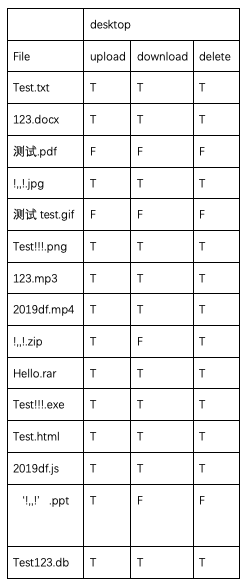
\includegraphics[width=60mm]{UDD.png}}%
\subfigure[Edit and Rename]{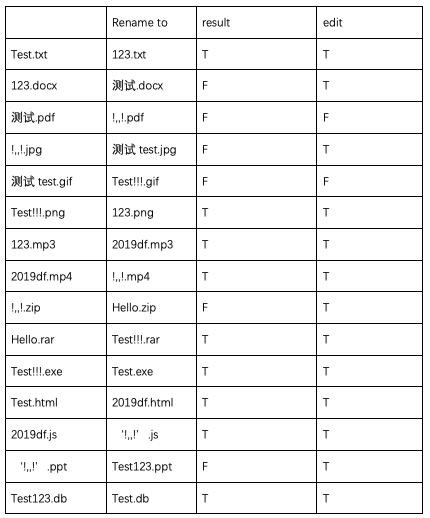
\includegraphics[width=60mm]{Rename.png}}
\end{figure}

The test case results for Mobile Client are as shown. Adding files are not as simple on Mobile as it is on Desktop and thus, the test cases are different:\newline

\begin{figure}[H]
\centering
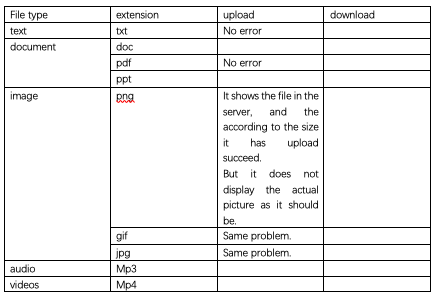
\includegraphics[scale=0.5]{mobiletest}
\end{figure}

\newline
\section{Team Contributions}

As mentioned, our development process was agile. All team members met for an hour on Thursday 1pm to communicate the progress of each sub-group and the plan for the next week. The main location is on the sixth floor of the Bush house SE building.   The meetings were also used to alleviate the difficulties encountered in our development process. The members of the group helped each other to solve these difficulties.\newline

The weekly meeting for Android is scheduled for Friday afternoon, and the desktop meeting is scheduled on Wednesday afternoon. WhatsApp was the chosen medium of informal communication. Independent progress was encouraged so as to not be slowed down by other members. All contributions raised through Pull requests on Git were reviewed by at least two other people to foster peer review and sharing of knowledge.\newline

Below are detailed accounts of the contribution of each member in the team (as written by the team members themselves) during project development process:\newline


\begin{figure}[ht]
\centering

\subfigure[Sivaranjani Subramanian]{
	\includegraphics[width=60mm]{siva.png}
}%
\subfigure[Letao Wang]{%
	\includegraphics[width=60mm]{Letao.png}
}

\end{figure}

\begin{figure}[H]
\centering

\subfigure[Qilin Zhou]{\includegraphics[width=60mm]{Qilin.png}}%
\subfigure[Lili Chen]{\includegraphics[width=60mm]{Lili.png}}

\caption{Commits and frequency graph of each member}

\end{figure}


\textbf{Georgii Fidarov:}
\begin{itemize}
\item Researched about edit button.
\item Researched about AWS Lambda.
\item Researched about Flutter.io.
\item Demonstrated Conflict scenarios and resolutions during preliminary presentation.
\end{itemize}

\textbf{Letao Wang:}
\begin{itemize}
\item Researched about Amazon S3.
\item Researched about using Electron and front-end language(HTML/Javascript) on S3.
\item Wrote “Tools/Technology” part in the initial report.
\item Demonstrated the basic functions of the desktop client in the initial presentation.
\item Implemented the basic function of Deadline Fighters desktop client with AWS S3 as server endpoint: Included upload one file, download a special file, delete a special file, rename a special file(Function removed upon further decisions).
\item Researched about delta sync, E-tag, MD5 and database.
\item Tried to implement the edit function with delta sync.
\item Researched about jQuery.
\item Implemented Deadline Fighters desktop client with AWS S3 as server endpoint: Included the download all files, upload all files, delete and download a special file(Function removed upon further decisions) for both server and local storage by using jQuery.
\item Designed the UI of the Deadline Fighters desktop client.
\item Designed the test case for both the desktop client and mobile client.
\item Test the test case for the desktop client.
\item Wrote “Implementation of the desktop client” and “Evaluation” part in the final report.
\end{itemize}


\textbf{Lili Chen:}
\begin{itemize}
\item Researched about using the electron and react-native to develop the desktop.
\item Wrote ‘what we have done so far’ and design the desktop UI in the initial report.
\item Research about how to using javascript and HTML with AWS S3.
\item Implemented Deadline Fighters desktop client with AWS S3 as server endpoint: Included the upload file to server and list file from the server to desktop.
\item Added CSS to the desktop.
\item Researched database for the desktop login page.
\item Researched Rsync algorithm for edit function
\item Researched about JQuery, font-awesome icon and bootstrap.
\item Researched jsunit test (mocha, sinon, chai) for desktop and try to implement it.
\item Done the black box test for the desktop.
\item Wrote ‘requirement and design’, ‘test case’ and ‘team works’ in the final report.
\end{itemize}


\textbf{Qilin Zhou:}
\begin{itemize}
\item Write ‘team protocol’ in the initial report.
\item Researched about using Flutter.io.
\item Researched the rsync algorithm.
\item Researched the unit test of Android and try to use it (not implemented yet).
\item Researched and compared different APIs provided by AWS SDK.
\item Researched the thread in Android development.
\item Implemented Deadline Fighters mobile client with AWS S3 as server endpoint: Included the download, upload, delete and rename(Function removed upon further decisions) for both server and local storage.
\item Worked with the desktop client team about the file listing and listener.
\item Researched about FileObserver and use FileObserver to detect the file status in the local storage.
\item Designed the UI of the Deadline Fighters mobile client.
\item Implemented Deadline Fighters mobile client with python server endpoint: Included the download, upload(Functions should be tested and improve).
\item Write the ‘mobile implementation’ in the final report.
\end{itemize}

\textbf{Sivaranjani Subramanian:}
\begin{itemize}
\item Single-handedly coded the Python server and migrated the entire Desktop client and its functionalities to communicate with the server as an enhancement over Letao and Lili's work that used S3 as server. Work included implementing boto3 SDK on Python for talking to AWS, understanding various ways of communication between server and client and implementing the three component framework (AWS, Server and Client) that Deadline fighters synchronizer now has, adding json encoding/decoding procedures as required and research/implementation of various HTTP requests on different platforms/languages.
\item Helped the team narrow down AWS services that can be used for the project. Set up and configured AWS account when Jacky had to leave the team.
\item Configured Git repo for the team. Functioned as the Git "expert" on the team, helping people deal with cherry-picking, merging during conflict, etc.
\item Added logging feature to all applications.
\item Formatted all code files involved to remove dead code, set uniform indentation etc.
\item Led brainstorming sessions on technology selection, conflict resolution, server implementation etc.
\item Major contributor to code reviews, commenting on functionality as well as best practices.
\item Helped co-ordinate meetings regularly by following up with team members. Letao helped when Sivaranjani had other commitments.
\item Helped collate and format both the preliminary presentation and final presentation. Work included proofreading, editing and formatting for better presentability.
\item Helped team members with the installation and usage of \LaTeX
\item Helped the team come to consensus using Google Forms, Doodle poll, meetings etc., as necessary.
\item \emph{Working on implementing the conflict resolution scenario at the time of this document submission.}
\end{itemize}



\section{Evaluation}

\subsection{Project Objectives}
Comparing the design part to the implementation part, here is a table of what design functions are worked and what are not:\newline
\begin{table}[H]
\centering
\begin{tabular}{|c|p{8cm}|p{2cm}|}
\hline
Operation & Object & Whether it is completed \\
\hline
\multirow{2}{*}{Upload}&{One file (May not in the local sync folder)}&Yes\\
\cline{2-3}
&All files in the local sync folder&Yes\\
\cline{1-3}
\multirow{2}{*}{Download}&{One file}&Yes\\
\cline{2-3}
&All files&Yes\\
\cline{1-3}
\multirow{2}{*}{Delete}&{One file}&Yes\\
\cline{2-3}
&All files&No\\
\cline{1-3}
\multirow{2}{*}{Rename}&{One file}&Yes\\
\cline{2-3}
&Two or more files&No\\
\cline{1-3}
\multirow{2}{*}{Edit}&{One file}&Yes\\
\cline{2-3}
&Two or more files&No\\
\cline{1-3}
\multirow{1}{*}{Synchronize}&{All files in the server and local syn folder}&Yes\\

\bottomrule
\end{tabular}
\caption{Current status of implementation}
\end{table}

\subsection{Team dynamics}
We have worked together in harmony for the most part of the project duration. Team size reduced during the week after the Preliminary report due to conflict. This not only led to redoing of some work but also added work load on the existing members. But the team managed to keep its morale through the whole process.\newline

One of the members had significantly less contributions compared to the rest of the team. This was amplified by lack of communication, attendance and general participation from the member. The gender skew of the team could be a possible reason for this.\newline

Also, sometimes, there was difficulty in communication due to the fact that more than 50\% of the team is Chinese.

The following is the distribution of 100 marks among members. Note that this was assigned with consensus of 4 members as the 5th member was absent on the day the marks were allocated:

\begin{table}[H]
\centering
\begin{tabular}{|c|c|}
\hline
Student Name &  Marks \\
\hline
Georgii Fidarov & 2 \\
\hline
Letao Wang & 24.5 \\
\hline
Lili Chen & 24.5 \\
\hline
Qilin Zhou & 24.5 \\
\hline
Sivaranjani Subramanian & 24.5 \\
\bottomrule
\end{tabular}
\caption{Mark distribution on team consensus}
\end{table}


}

\end{flushleft}




\end{document}
